\documentclass{l4proj}

%
%  Macro files
%  Originally from Frisch, Castagna, Benzaken
%  
%

%% Ornela
\newcommand{\abstr}[4]{\lambda_{({#1} , {#2})} {#3}.{#4}}
\newcommand{\semval}[2]{\sem{#1}_{\mathcal #2}}



\newif{\ifSHORT}
\newif{\ifLongVersion}
\newif{\ifWithRecords}
\newif{\ifWiths}

\newcommand{\possiblecut}[1]{{\color{black}#1}}   

\newcommand{\maincomment}[1]{%
  \ifMarginalComments{\mbox{}\\[1mm]$\Longrightarrow$\textsf{#1}\mbox{}\\[1mm]} \else {} \fi}

\newenvironment{mylist}{%
\begin{list}{$\bullet$}{\topsep2pt\parskip0pt\partopsep0pt\itemsep3pt\labelwidth10.5mm\labelsep3pt\leftmargin11mm}}%
{\end{list}}

%
%  unsemplice comando che mi dice la versione
%
\usepackage{calc}\newcounter{tempo}\setcounter{tempo}{\time}
\newcommand{\version}[1]{\mbox{}\\[-\baselineskip]%
   \raisebox{#1in}[0in][0in]{\makebox[\textwidth][c]{\rm\small \today:v.\thetempo}}}
\newcommand{\titlepageheader}[1]{\mbox{}\\[-\baselineskip]%
\raisebox{5.3in}[0in][0in]{\makebox[\textwidth][c]{\rm\small #1}}}
\newcommand{\duce}{$\mathbb{C}$Duce }
\newcommand{\cduce}{$\mathbb{C}$Duce }
\newcommand{\cdoge}{$\mathbb{C}$Doge }
\newcommand{\cpi}{$\mathbb{C}\pi$ }
\newcommand{\cobj}{$\mathbb{C}$Obj }
\newcommand{\sempi}{$\pi_\leq$}   % was semantic-$\pi${}}
\newcommand{\emptyl}{\mathsf{empty}}
%
% Daniele
%
% altri commandi
\newcommand{\wt}[1]{\widetilde{#1}}

\newcommand{\synrnd}{\mathbf{rnd}}
\newcommand{\synclass}{\mathbf{class} \ }
\newcommand{\syninterface}{\mathbf{interface} \ }
\newcommand{\synext}{\ \mathbf{extends }\ }
\newcommand{\synimpl}{\ \mathbf{implements}\ }
\newcommand{\synret}{\mathbf{return}\ }
\newcommand{\synthis}{\mathbf{this}}
\newcommand{\synsuper}{\mathbf{super}}
\newcommand{\synfinal}{\mathbf{final}}
\newcommand{\synnew}{\mathbf{new}\ }
\newcommand{\syndecl}[3]{\synclass #1 \synext #2\ \{#3\}}
\newcommand{\synidecl}[2]{\synclass #1 \synext #2\ }

\newcommand{\mmif}{\mathbf{if}}
\newcommand{\mmthen}{\mathbf{then}}
\newcommand{\mmelse}{\mathbf{else}}
\newcommand{\mmclass}{\mathbf{class}}
\newcommand{\mmnew}{\mathbf{new}}
\newcommand{\mmnull}{\mathbf{null}}
\newcommand{\mmextends}{\mathbf{extends}}
\newcommand{\mmint}{\mathbf{int}}
\newcommand{\mmreal}{\mathbf{real}}
\newcommand{\mmbool}{\mathbf{bool}}
\newcommand{\mmtrue}{\mathbf{true}}
\newcommand{\mmfalse}{\mathbf{false}}
\newcommand{\nname}{\mathbf{name}}
\newcommand{\mmreturn}{\mathbf{return}}
\newcommand{\mminstof}{\mathbf{instanceof}}
\newcommand{\mmtry}{\mathbf{try}}
\newcommand{\mmcatch}{\mathbf{catch}}
\newcommand{\mmthrow}{\mathbf{throw}}
\newcommand{\mmlet}{\mathbf{let}}
\newcommand{\mmin}{\mathbf{in}}
\newcommand{\nominal}{\mathbf{nominal}}

\newcommand{\naming}[1]{(#1)^\nname}
\newcommand{\type}{\mathit{type}}
\newcommand{\mbody}{\mathit{body}}
\newcommand{\judge}[2]{#1 \vdash #2}
\newif\ifmai\maifalse


\newcommand{\height}[1]{\hslash(#1)}%{\textit{height}(#1)}
%\DeclareMathOperator{\uparrowop}{\uparrow}
%\DeclareMathOperator{\downarrowop}{\downarrow}
%
% definition enum environment
%
\newenvironment{enum}{\begin{enumerate}\vspace{-5pt}\topsep0pt\parskip0pt\partopsep0pt\itemsep1pt}{\end{enumerate}\vspace{-5pt}}


%
%
\newcommand{\A}{{\cal A}}
\newcommand{\Norm}{{\cal N}}
\newcommand{\exten}{\mathbb E}
\newcommand{\extenf}{\mathbb{E}_f}
\newcommand{\atoms}{{\mathbb T}}
\newcommand{\myitem}{\mbox{}\\[.5mm]\hspace*{3.5mm}--~~}

\newcommand{\dead}{\textsf{0}}
%\newcommand{\mathbb}[1]{\Bbb{#1}}
%\newcommand{\llbracket}{[\![}
%\newcommand{\rrbracket}{]\!]}

\newcommand{\VAR}{\textit{Var}}
\newcommand{\zero}{\mathbf{0}}
\newcommand{\one}{\mathbf{1}}
%\newcommand{\qed}{\mbox{}\hfill\mbox{$\Box$}}
\newcommand{\bij}{\partial}
\newcommand{\para}{~~|~~}
\newcommand{\hasse}[1]{\xymatrix@R-1em@C-2em{#1}}

\newcommand{\todo}[1]{{\bf \underline{TODO:} #1}}
\newcommand{\ignore}[1]{}
\newcommand{\Is}{\colon\!\!\colon \!\!\!\!= }

\newcommand{\txtvee}{\text{\rm ~or~}}
\newcommand{\txtwedge}{\text{\rm ~and~}}

\newcommand{\dom}{\textit{dom}}

%\newcommand{\naturals}{\mathbb{N}}

% Op�rateurs math�matiques
\renewcommand{\P}{{\cal P}}
\newcommand{\Pf}{{\P_f}}
\newcommand{\compl}[2]{{\complement_{#2}} {#1}}
\newcommand{\egdef}{\stackrel{\textrm{\tiny def}}{=}}
\newcommand{\segdef}{\!\!\!\stackrel{\textrm{\tiny def}}{=}\!\!\!}
\renewcommand{\subset}{\subseteq}
\renewcommand{\emptyset}{\varnothing}

\newcommand{\cX}{{\cal X}}

% Les univers
\newcommand{\ubasic}{{\text{\bf basic}}}
\newcommand{\urec}{{\text{\bf rec}}}
\newcommand{\ufun}{{\text{\bf fun}}}

% Basic types
\newcommand{\btypes}{{\mathbb B}}
\newcommand{\semb}[1]{{\cal B} {\llbracket #1 \rrbracket}}
\newcommand{\Types}{\textbf{Types}}
% Les mod�les
\newcommand{\domaine}{{\cal D}}
%\newcommand{\univ}{{\cal U}}
\newcommand{\domwr}{\domaine_\Omega}
\newcommand{\stdmod}{{\cal U}}
\newcommand{\stdmodwr}{{\cal U}_\Omega}
\newcommand{\sem}[1]{{\llbracket #1 \rrbracket}}
\newcommand{\esem}[1]{{\mathbb E}\left( #1 \right)}
\newcommand{\esemd}[1]{{\mathbb E}$D$}
\newcommand{\esemp}[1]{{\cal E}\llparenthesis #1 \rrparenthesis}
\newcommand{\tsem}[1]{\llparenthesis #1 \rrparenthesis}
%\newcommand{\semv}[1]{{\mathbb V}{\llbracket #1 \rrbracket}}


% Les types
\newcommand{\functor}{{\mathbb T}}
\newcommand{\syntypes}{{\mathcal{T}}}
\newcommand{\atomtypes}{\textit{A\/}}%{\syntypes^\circ}
\newcommand{\synatoms}{{\mathcal A}}
\newcommand{\synprod}{\pmb{\times}}
\newcommand{\synarrow}{\pmb{\rightarrow}}
\newcommand{\synneg}{\pmb{\neg}}
\newcommand{\synvee}{\pmb{\vee}}
\newcommand{\synwedge}{\pmb{\wedge}}
\newcommand{\syndiff}{\pmb{\backslash}}
\newcommand{\syncap}{\operatornamewithlimits{\pmb{\bigwedge}}}
\newcommand{\syncup}{\operatornamewithlimits{\pmb{\bigvee}}}
\newcommand{\socle}[1]{\beth(#1)}
\newcommand{\appl}{\bullet}
\newcommand{\synch}[2]{\textit{ch}^{#1}\!(#2)}
\newcommand{\synchan}[1]{\textit{ch}(#1)}
\newcommand{\synchanK}{\textit{ch}}
\newcommand{\synchanout}[1]{\textit{ch}^{\!\textbf{--}\!\!}(#1)}
\newcommand{\synchanin}[1]{\textit{ch}^+(#1)}

%blackboardbold types
\def\bbbone{{\mathchoice {\rm 1\mskip-4mu l} {\rm 1\mskip-4.5mu l}
          {\rm 1\mskip-4.5mu l} {\rm 1\mskip-5mu l}}}
\newcommand{\synnatone}{\bbbone}
\newcommand{\synnatk}{\Bbbk}
\newcommand{\synnat}[1]{\mathbb{#1}}

% Les motifs
\newcommand{\pator}[2]{#1 \pmb{|} #2}
\newcommand{\patand}[2]{#1 \pmb{\wedge} #2}
%\newcommand{\patleft}[1]{\pmb{(}#1\pmb{,\_)}}
%\newcommand{\patright}[1]{\pmb{(\_,}#1\pmb{)}}
\newcommand{\patcst}[2]{\pmb{(}#1\pmb{:=}#2\pmb{)}}
\newcommand{\patpair}[2]{\pmb{(}#1\pmb{,}#2\pmb{)}}

% Filtrage
\newcommand{\erreur}{\Omega}
\newcommand{\accept}[1]{\pmb{\lbag} #1 \pmb{\rbag}}
\newcommand{\acceptd}[1]{\pmb{\lfloor} #1 \pmb{\rfloor}}
\newcommand{\semaccept}[1]{\Lbag #1 \Rbag}
\newcommand{\filter}[2]{({#1}/{#2})}%{ ({#1} \Downarrow {#2}) }
\newcommand{\semfilter}[2]{ ({#1} \downarrow {#2}) }


% Symboles du langage
%\newcommand{\myarrow}{\Pisymbol{cmt}{61}\Pisymbol{pcr}{62}}%
\newcommand{\myarrow}{\!\!\boldsymbol{\Rightarrow}\!\!} %\texttt{\char61\char62\relax}}
\newcommand{\mybar}{\texttt{|}}%
\newcommand{\motifs}{\mathbb{P}}
\newcommand{\vars}{\mathbb{V}}
\newcommand{\consts}{\mathbb{C}}
\newcommand{\exprs}{{\mathbb E}}
\newcommand{\expr}{{e}}
\newcommand{\pat}{{\tt p}}
\newcommand{\const}{{n}}
\newcommand{\op}{{o}}
\newcommand{\ops}{{\mathbb O}}
\newcommand{\valeurs}{{\cal V}}
\newcommand{\values}{\valeurs}
\newcommand{\blpar}{\boldsymbol{(}}
\newcommand{\brpar}{\boldsymbol{)}}
\newcommand{\match}[5]{\mathtt{match~} #1 \mathtt{~with~} #2 \myarrow #3 \mybar
  #4 \myarrow #5}
\newcommand{\typecase}[5]{\mathtt{typecase~} #1 \mathtt{~with~} (#2 :
  #3) \myarrow #4 \mybar (#2 : \synneg #3) \myarrow #5}
\newcommand{\typec}[5]{\texttt{(} #3=#1\pmb{\in}#2\texttt{)}\pmb{?}#4\texttt{{:}}#5}
\newcommand{\genabstraction}[3]{\abstr{f}{#1}{#2}{#3}}
%\newcommand{\abstr}[4]{\boldsymbol{\mu} #1^{\blpar #2 \brpar}\blpar #3 \brpar \boldsymbol{.}#4}
\newcommand{\stdmatch}{\match{\expr}{p_1}{\expr_1}{p_2}{\expr_2}}
\newcommand{\exprpair}[2]{\blpar #1 \boldsymbol{,} #2 \brpar}
\newcommand{\exprop}[2]{#1 \blpar #2 \brpar}

% S�mantique op�rationnelle
%\newcommand{\wrong}{\mbox{\bf wrong}}
\newcommand{\wrong}{\Omega}
%\newcommand{\reject}{\mbox{\bf reject}}
%\newcommand{\apply}{{\tt apply}}


% Enregistrements
\newcommand{\domdef}[1]{\text{Def}(#1)}
\newcommand{\labels}{{\cal L}}
\newcommand{\urecord}{{\text{\bf record}}}
\newcommand{\trec}[2]{\pmb{[} #1 : #2 \pmb{]}}
\newcommand{\tsupp}[1]{\text{\bf S}(#1)}
%\newcommand{\supp}[1]{\text{Supp}(#1)}
\newcommand{\patrec}[2]{\{ #1 : #2\}}
\newcommand{\Iff}{\Longleftrightarrow}
\newcommand{\reff}{\mathtt{ref}\,}
\newcommand{\lazy}{\mathtt{lazy}\,}


% Th�or�mes ...
%\newtheorem{theorem}{Theorem}[section]
%\newtheorem{lemma}[theorem]{Lemma}
%\newtheorem{proposition}[theorem]{Proposition}
%\newtheorem{corollary}[theorem]{Corollary}
%\newtheorem{definition}[theorem]{Definition}
%\newtheorem{condition}{Condition}
%\newenvironment{definition}{\begin{defn}}{\qed\end{defn}}
%\newtheorem{definition}[theorem]{Definition}
%\newtheorem{property}[theorem]{Property}
%\newtheorem{convention}[theorem]{Convention}
%\newtheorem{remark}[theorem]{Remark}
%\renewenvironment{proof}{{\sl Proof}:}{\qed}


\begin{document}

%===================================================================================================

\title{Boolean types and semantic subtyping for Featherweight Java}
\author{Artem Usov}
\date{January 18, 2020}

\maketitle

%===================================================================================================

\begin{abstract}
    Every abstract follows a similar pattern. Motivate; set aims; describe work; explain results.
    \vskip 0.5em
    ``XYZ is bad. This project investigated ABC to determine if it was better.
    ABC used XXX and YYY to implement ZZZ. This is particularly interesting as XXX and YYY have
    never been used together. It was found that
    ABC was 20\% better than XYZ, though it caused rabies in half of subjects.''
\end{abstract}

%===================================================================================================

\def\consentname {Artem Usov}
\def\consentdate {19 January 2020}
\educationalconsent

%===================================================================================================

\tableofcontents

%===================================================================================================

\chapter{Introduction}

\pagenumbering{arabic}

\section{End goal of programming}

The end goal in all programming projects, is to create a solution to the task at hand that performs exactly as expected by the programmer, and exactly solves the problem that was initially defined.
However, this very rarely actually happens.

On the one hand, this is often because the original problem is not statically defined.
If it is a solution for an external client, their requirements and needs will change over time, or the needs and wants of the users using this project can also change.
This means the project needs to be adapted over time.
On the other hand, and almost always much less evident, is that programs do not perform exactly as the programmer imagines them to work.

These are in general called \emph{bugs} in a program, and have become more and more common as the projects we create have become more complex compared to the early days of computing and the underlying hardware we work on has also become more complex.
Therefore in both academia and industry, there have been great efforts over the years to create tools that allow us to decrease the amount of bugs in our programs and increase our productivity.

\subsection{Static Code Analysis}

One area of great effort has been in the development of static code analysis tools.
Some of these exist integrated into the language itself such as with Spark \citep{Carre1990}.
Spark is a formally defined language based on the Ada \citep{Ada1979} language intended for the development of high integrity software such as flight control systems.
Spark uses contracts and flow analysis to logically prove that programs are correct.
Others exist as separate, well-known tools that exist alongside the language such as the Clang analysis tools for C and C++ \citep{kremenek2008}.

While they are not necessarily needed to write correct programs, these tools have quickly become industry standards for maintaining a level of correctness within codebases and avoiding typical programming errors.

\subsection{Into Static Analysis}

Underlying all of the previously mentioned static code analysis tools, is their use of the \textbf{type system} of the language.
Type systems at their most basic work by assigning types to various constructs of a program so that incompatible types cannot be used.

For example, one common area of error in C code that the Clang tools warn about is implicit conversions where the value of an expression is a different type from the one expected, such as the use of a floating point number where an integer is expected.
The C language will implicitly convert the value to an integer, however this can cause unexpected behaviour for the programmer.
It knows that this conversion needs to happen as the type system dictates that you cannot use any other type other than an integer where an integer is expected.

\section{Varying Type Systems}

The effectiveness of static analysis tools and more generally the \emph{safety} and \emph{expressivity} of a programming language therefore depends on the type system that is used.
Type systems have evolved from the relatively simple systems in languages like C to more complex ones such as in Java where there are custom object types and subtyping relations where types can be substituted for one another.

More modern advances in type systems include the use of linear types in the Cyclone \citep{grossman2002} language that allow us to more naturally and logically define finite state machines.
There exist other new developments in type systems such as Boolean types which are explored in this paper.

\section{Goals of this Project}

In this section, the issue and aims of this paper are presented.

\subsection{Problem Statement}

The typical hierarchical subtyping definitions in Java quite often restrict and complicate the logic that the programmer wants to implement. These problems come up particularly often when working with legacy code that has defines incorrect abstractions in its classes. This therefore leads to less understandable and less maintainable code, that could cause problems in the future.

\subsection{Aims}

The aim of this project is to implement a new programming language that uses a proposed type system consisting of boolean types and a semantic subtyping algorithm. This project aims to transform the mathematical definition of such a type system into an actual solution in software, solving the issues encountered doing so. The language should be able to illustrate the improved solutions to the
common example problems encounter in a language without these features such as Java. Furthermore, the language will be evaluated so see whether these additional language features are intuitive to use by programmers.

\section{Dissertation Outline}

The dissertation is structured into seven chapters as follow:

\begin{itemize}
    \item
          \textbf{Chapter 2} provides background about type systems and Featherweight Java, the language on top of which the new type system is implemented. We also discuss some existing work on semantic type systems and boolean types.
    \item
          \textbf{Chapter 3} TODO
    \item
          \textbf{Chapter 4} TODO
    \item
          \textbf{Chapter 5} TODO
    \item
          \textbf{Chapter 6} contains details about the evaluation method, evaluation results and analysis of results.
    \item
          Finally \textbf{chapter 8} concludes the dissertation with a summary of the important results.
\end{itemize}

%===================================================================================================

\chapter{Background}


\section{Type Systems}

In all modern programming languages, a type systems is arguably the main way that incorrect behaviour in a program is reduced.
A possible definition of a type system is given by \citet{Pierce2002} as:

\emph{A type system is a tractable syntactic method for proving the absence of certain program behaviors by classifying phrases according to the kinds of values they compute.}

In particular, the most important detail in the above definition is the emphasis on classifying phrases in our language into a particular type based on the kinds of values they hold or compute.
For example by using a type system, we can check that the arguments given to an arithmetic operation are always numbers.
Therefore we can validate that a specific program is absent of certain bad run-time behaviour such as trying to add a boolean value \emph{true} to a number \emph{2}.

However what the above definition is inaccurate about is that is it defines a type system to be solely a syntactic method, in which the system is defined as a list of formal deduction rules.
The syntactic approach is certainly by far the most common approach for a type system.
However, there does exist an alternative method in the semantic approach.
\citet{Frisch2002} describe the semantic approach as instead starting with a model of the language and all the possible values in the language and defines an interpretation of types as subsets of values the model.

Such as model comes with several advantages.
For example, given two types $s$ and $t$, which represent a certain subset of values in the model, when $s \subseteq t$ does not hold, then it is possible to exhibit an element of the model which is in the interpretation of type $s$ and not $t$.
This can then be used to show more informative error messages to the programmer \citep{Castagna2005}, such as showing which value in $s$ is causing the equality not to hold.
However due to being a more technical approach, such as the non-triviality of defining the interpretation of types as subsets of a model, the semantic method has received less attention than syntactic methods.

The first problem we encounter in the semantic approach is that in such a model, $t_{1}$ is a subtype of $t_{2}$ if all the $t_{1}$-values are also $t_{2}$-values, i.e. the equality $t_{1} \subseteq t_{2}$ holds.
However, in this way, subtyping is defined by relying on the notion of well-typed values; hence, we need the typing relation to determine typing judgements for values; but the typing rules use the subtyping relation defined in \citep{Dardha2017}.
So, there is a circularity in our definition, as demonstrated in Figure \ref{fig:circ}.

To solve this problem, we follow the framework defined by \citet{Frisch2008}.
The general idea of the framework is that we first extend the types in the language with \emph{Boolean Combinators}: union $\lor$, intersection $\land$ and negation $\neg$.
We can then define an abstract model $\beta$ where our types are interpreted according to the set-theoretic meaning of the combinators and can define subtyping as set-inclusion and therefore define the typing rules.
Separately, if we have a notion of well-typed values, we can define another interpretation of types as sets of values.
We can again define a subtyping relation $\nu$.
While these may be different relation, if the models are chosen carefully such that:
\begin{equation*}
    s \leq_{\beta} t \iff s \leq_{\nu} t,
\end{equation*}

then these models coincide and this closes the circularity.

\begin{figure}
    \centering
    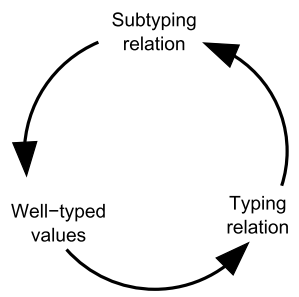
\includegraphics[width=0.4\linewidth]{images/circularity.PNG}
    \caption{Circularity in the semantic subtyping definition \citep{Castagna2005}}
    \label{fig:circ}
\end{figure}

\section{Featherweight Java}

The syntax of the JSF is exactly that of Featherweight Java (FJ) \citep{Igarashi1999}, with only the associated type system being different.
This was chosen on purpose as the full features of Java such as concurrency and reflection are orthogonal to the purpose of demonstrating the use of the novel semantic type system.
The main key simplification in FJ from Java is the omission of assignment.
All fields of an object cannot be changed after initialisation and all methods are pure functions
While this restricts FJ to what is essentially a functional fragment of Java, it is still fully computationally complete.

\section{Tools}

The type system of FSJ was built using Antlr to define the grammar and type checking of the language and the


\section{Related Work}
The closest similar area of research would likely be the work on $\mathbb{C}$Duce
\citep{Benzaken2003}, which is also a functional language with a semantic type system designed for
working with XML documents and a continuation of the work on XDuce \citep{Hosoya2003}. The language
extended XDuce by introducing less XML specific types such as records, boolean connectives and arrow
types. This therefore makes it similar to (\textit{TODO reword}) our language in that a class-based
semantic type system is a combination of the $\mathbb{C}$Duce record types with arrow types
\textit{(fields and methods)}

Our work and the work on $\mathbb{C}$Duce follow the functional style of $\lambda$-calculus,
whereas the work by \citet{Castagna2008} extends $\pi$-calculus with semantic subtyping.
(\textit{TODO reword}) Similar work to ours creating an implementation for this would result in a
Golang-like language \citep{Meyerson2014}, creating a concurrency-focused language with more
intuitive types. The paper found that it was required to be able to decide and resolve the atomicy,
that is whether the only proper subtype is the empty type, of types in order to decide the subtyping
relation, and observes that this same problem appears in $\lambda$-calculus and any other
semantic-based system, for which we will show where we encountered this problem further in this
paper.

%==================================================================================================================================
\chapter{Analysis/Requirements}
What is the problem that you want to solve, and how did you arrive at it?
\section{Guidance}
Make it clear how you derived the constrained form of your problem via a clear and logical process.

%==================================================================================================================================
\chapter{Design}
How is this problem to be approached, without reference to specific implementation details?


\label{sec:design}
The syntax of types is given by the following grammar \citep{Dardha2013,Dardha2017}:
$$
    \begin{array}{llll}
        \tau   & ::=                                       & \alpha \ |\ \mu
               & \mbox{{\em Type term}}
        \\
        \alpha & ::=                                       & \zero \ |\ \btypes \ |\ [\wt{l:\tau}] \ |\ \alpha \ \bf{and}\ \alpha \ |\ \bf{not}\ \alpha
        \qquad
               & \mbox{{\em Object type} ($\alpha $-type)}
        \\
        \mu    & ::=                                       & \alpha \to \alpha \ |\ \mu \ \bf{and}\ \mu \ |\ \bf{not}\ \mu
               & \mbox{{\em Method type} ($\mu $-type)}
    \end{array}
$$

The syntax of terms is given by the following grammar and is based on the standard syntax of terms in FJ \cite{Igarashi1999,Dardha2013,Dardha2017}:
\begin{align*}
     & \mbox{\textit{Class declaration}}  & L \; ::= \; & \syndecl{C}{C}{\wt{\alpha \ a};\ K; \ \wt{M}\ }                         \\
     & \mbox{\textit{Constructor}}        & K \;::=\;   & C\ (\wt{\alpha\ x})\ \{\ \synsuper(\wt{x});\ \wt{\synthis.a}=\wt{x}; \} \\
     & \mbox{\textit{Method declaration}} & M \; ::= \; & \alpha \ m\ (\alpha \ x)\ \{\ \synret e; \}                             \\
     & \mbox{\textit{Expressions}}        & e \; ::=\;  & x\ |\  c\ |\ e.a\ |\ e.m(e) \ | \ \synnew C(\wt{e})
\end{align*}

\begin{figure}
    \centering
    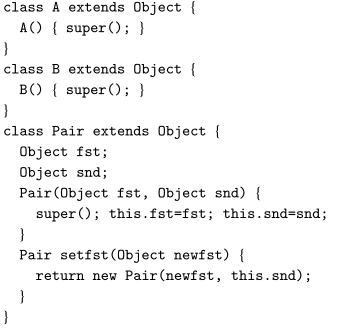
\includegraphics[width=0.4\linewidth]{images/class.PNG}
    \caption{TODO caption, \citep{Igarashi1999}}
    \label{fig:class}
\end{figure}

\section{Guidance}
Design should cover the abstract design in such a way that someone else might be able to do what you did, but with a different language or library or tool.

%==================================================================================================================================
\chapter{Implementation}
What did you do to implement this idea, and what technical achievements did you make?
\section{Guidance}
You can't talk about everything. Cover the high level first, then cover important, relevant or impressive details.



\section{General points}

These points apply to the whole dissertation, not just this chapter.



\subsection{Figures}
\emph{Always} refer to figures included, like Figure \ref{fig:relu}, in the body of the text. Include full, explanatory captions and make sure the figures look good on the page.
You may include multiple figures in one float, as in Figure \ref{fig:synthetic}, using \texttt{subcaption}, which is enabled in the template.



% Figures are important. Use them well.
\begin{figure}
    \centering
    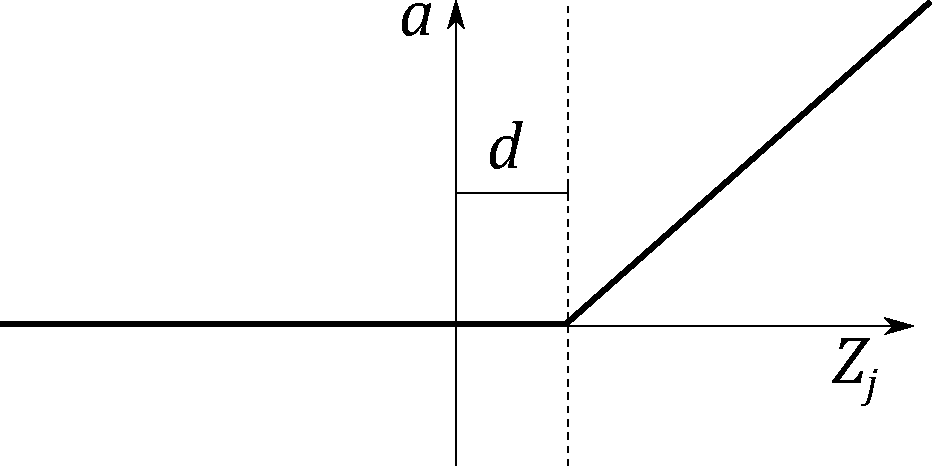
\includegraphics[width=0.5\linewidth]{images/relu.pdf}
    
    \caption{In figure captions, explain what the reader is looking at: ``A schematic of the rectifying linear unit, where $a$ is the output amplitude,
        $d$ is a configurable dead-zone, and $Z_j$ is the input signal'', as well as why the reader is looking at this:
        ``It is notable that there is no activation \emph{at all} below 0, which explains our initial results.''
        \textbf{Use vector image formats (.pdf) where possible}. Size figures appropriately, and do not make them over-large or too small to read.
    }
    
    % use the notation fig:name to cross reference a figure
    \label{fig:relu}
\end{figure}


\begin{figure}
    \centering
    \begin{subfigure}[b]{0.45\textwidth}
        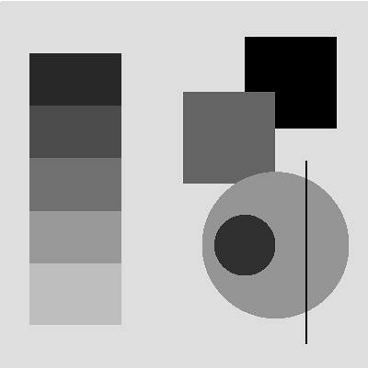
\includegraphics[width=\textwidth]{images/synthetic.png}
        \caption{Synthetic image, black on white.}
        \label{fig:syn1}
    \end{subfigure}
    ~ %add desired spacing between images, e. g. ~, \quad, \qquad, \hfill etc.
    %(or a blank line to force the subfigure onto a new line)
    \begin{subfigure}[b]{0.45\textwidth}
        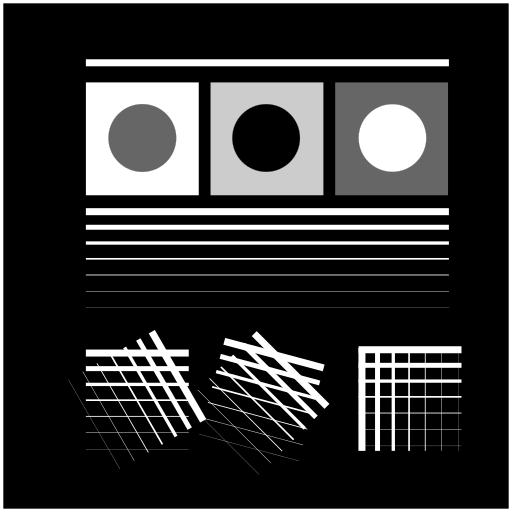
\includegraphics[width=\textwidth]{images/synthetic_2.png}
        \caption{Synthetic image, white on black.}
        \label{fig:syn2}
    \end{subfigure}
    ~ %add desired spacing between images, e. g. ~, \quad, \qquad, \hfill etc.
    %(or a blank line to force the subfigure onto a new line)
    \caption{Synthetic test images for edge detection algorithms. \subref{fig:syn1} shows various gray levels that require an adaptive algorithm. \subref{fig:syn2}
        shows more challenging edge detection tests that have crossing lines. Fusing these into full segments typically requires algorithms like the Hough transform.
        This is an example of using subfigures, with \texttt{subref}s in the caption.
    }\label{fig:synthetic}
\end{figure}

\clearpage

\subsection{Equations}

Equations should be typeset correctly and precisely. Make sure you get parenthesis sizing correct, and punctuate equations correctly
(the comma is important and goes \textit{inside} the equation block). Explain any symbols used clearly if not defined earlier.

For example, we might define:
\begin{equation}
    \hat{f}(\xi) = \frac{1}{2}\left[ \int_{-\infty}^{\infty} f(x) e^{2\pi i x \xi} \right],
\end{equation}
where $\hat{f}(\xi)$ is the Fourier transform of the time domain signal $f(x)$.

\subsection{Algorithms}
Algorithms can be set using \texttt{algorithm2e}, as in Algorithm \ref{alg:metropolis}.

% NOTE: line ends are denoted by \; in algorithm2e
\begin{algorithm}
    \DontPrintSemicolon
    \KwData{$f_X(x)$, a probability density function returing the density at $x$.\; $\sigma$ a standard deviation specifying the spread of the proposal distribution.\;
        $x_0$, an initial starting condition.}
    \KwResult{$s=[x_1, x_2, \dots, x_n]$, $n$ samples approximately drawn from a distribution with PDF $f_X(x)$.}
    \Begin{
        $s \longleftarrow []$\;
        $p \longleftarrow f_X(x)$\;
        $i \longleftarrow 0$\;
        \While{$i < n$}
        {
            $x^\prime \longleftarrow \mathcal{N}(x, \sigma^2)$\;
            $p^\prime \longleftarrow f_X(x^\prime)$\;
            $a \longleftarrow \frac{p^\prime}{p}$\;
            $r \longleftarrow U(0,1)$\;
            \If{$r<a$}
            {
                $x \longleftarrow x^\prime$\;
                $p \longleftarrow f_X(x)$\;
                $i \longleftarrow i+1$\;
                append $x$ to $s$\;
            }
        }
    }
    
    \caption{The Metropolis-Hastings MCMC algorithm for drawing samples from arbitrary probability distributions,
        specialised for normal proposal distributions $q(x^\prime|x) = \mathcal{N}(x, \sigma^2)$. The symmetry of the normal distribution means the acceptance rule takes the simplified form.}\label{alg:metropolis}
\end{algorithm}

\subsection{Tables}

If you need to include tables, like Table \ref{tab:operators}, use a tool like https://www.tablesgenerator.com/ to generate the table as it is
extremely tedious otherwise.

\begin{table}[]
    \caption{The standard table of operators in Python, along with their functional equivalents from the \texttt{operator} package. Note that table
        captions go above the table, not below. Do not add additional rules/lines to tables. }\label{tab:operators}
    %\tt
    \rowcolors{2}{}{gray!3}
    \begin{tabular}{@{}lll@{}}
        %\toprule
        \textbf{Operation}    & \textbf{Syntax}                         & \textbf{Function}                          \\ %\midrule % optional rule for header
        Addition              & \texttt{a + b}                          & \texttt{add(a, b)}                         \\
        Concatenation         & \texttt{seq1 + seq2}                    & \texttt{concat(seq1, seq2)}                \\
        Containment Test      & \texttt{obj in seq}                     & \texttt{contains(seq, obj)}                \\
        Division              & \texttt{a / b}                          & \texttt{div(a, b) }                        \\
        Division              & \texttt{a / b}                          & \texttt{truediv(a, b) }                    \\
        Division              & \texttt{a // b}                         & \texttt{floordiv(a, b)}                    \\
        Bitwise And           & \texttt{a \& b}                         & \texttt{and\_(a, b)}                       \\
        Bitwise Exclusive Or  & \texttt{a \textasciicircum b}           & \texttt{xor(a, b)}                         \\
        Bitwise Inversion     & \texttt{$\sim$a}                        & \texttt{invert(a)}                         \\
        Bitwise Or            & \texttt{a | b}                          & \texttt{or\_(a, b)}                        \\
        Exponentiation        & \texttt{a ** b}                         & \texttt{pow(a, b)}                         \\
        Identity              & \texttt{a is b}                         & \texttt{is\_(a, b)}                        \\
        Identity              & \texttt{a is not b}                     & \texttt{is\_not(a, b)}                     \\
        Indexed Assignment    & \texttt{obj{[}k{]} = v}                 & \texttt{setitem(obj, k, v)}                \\
        Indexed Deletion      & \texttt{del obj{[}k{]}}                 & \texttt{delitem(obj, k)}                   \\
        Indexing              & \texttt{obj{[}k{]}}                     & \texttt{getitem(obj, k)}                   \\
        Left Shift            & \texttt{a \textless{}\textless b}       & \texttt{lshift(a, b)}                      \\
        Modulo                & \texttt{a \% b}                         & \texttt{mod(a, b)}                         \\
        Multiplication        & \texttt{a * b}                          & \texttt{mul(a, b)}                         \\
        Negation (Arithmetic) & \texttt{- a}                            & \texttt{neg(a)}                            \\
        Negation (Logical)    & \texttt{not a}                          & \texttt{not\_(a)}                          \\
        Positive              & \texttt{+ a}                            & \texttt{pos(a)}                            \\
        Right Shift           & \texttt{a \textgreater{}\textgreater b} & \texttt{rshift(a, b)}                      \\
        Sequence Repetition   & \texttt{seq * i}                        & \texttt{repeat(seq, i)}                    \\
        Slice Assignment      & \texttt{seq{[}i:j{]} = values}          & \texttt{setitem(seq, slice(i, j), values)} \\
        Slice Deletion        & \texttt{del seq{[}i:j{]}}               & \texttt{delitem(seq, slice(i, j))}         \\
        Slicing               & \texttt{seq{[}i:j{]}}                   & \texttt{getitem(seq, slice(i, j))}         \\
        String Formatting     & \texttt{s \% obj}                       & \texttt{mod(s, obj)}                       \\
        Subtraction           & \texttt{a - b}                          & \texttt{sub(a, b)}                         \\
        Truth Test            & \texttt{obj}                            & \texttt{truth(obj)}                        \\
        Ordering              & \texttt{a \textless b}                  & \texttt{lt(a, b)}                          \\
        Ordering              & \texttt{a \textless{}= b}               & \texttt{le(a, b)}                          \\
        % \bottomrule
    \end{tabular}
\end{table}
\subsection{Code}

Avoid putting large blocks of code in the report (more than a page in one block, for example). Use syntax highlighting if possible, as in Listing \ref{lst:callahan}.

\begin{lstlisting}[language=python, float, caption={The algorithm for packing the $3\times 3$ outer-totalistic binary CA successor rule into a
    $16\times 16\times 16\times 16$ 4 bit lookup table, running an equivalent, notionally 16-state $2\times 2$ CA.}, label=lst:callahan]
    def create_callahan_table(rule="b3s23"):
        """Generate the lookup table for the cells."""
        s_table = np.zeros((16, 16, 16, 16), dtype=np.uint8)
        birth, survive = parse_rule(rule)

        # generate all 16 bit strings
        for iv in range(65536):
            bv = [(iv >> z) & 1 for z in range(16)]
            a, b, c, d, e, f, g, h, i, j, k, l, m, n, o, p = bv

            # compute next state of the inner 2x2
            nw = apply_rule(f, a, b, c, e, g, i, j, k)
            ne = apply_rule(g, b, c, d, f, h, j, k, l)
            sw = apply_rule(j, e, f, g, i, k, m, n, o)
            se = apply_rule(k, f, g, h, j, l, n, o, p)

            # compute the index of this 4x4
            nw_code = a | (b << 1) | (e << 2) | (f << 3)
            ne_code = c | (d << 1) | (g << 2) | (h << 3)
            sw_code = i | (j << 1) | (m << 2) | (n << 3)
            se_code = k | (l << 1) | (o << 2) | (p << 3)

            # compute the state for the 2x2
            next_code = nw | (ne << 1) | (sw << 2) | (se << 3)

            # get the 4x4 index, and write into the table
            s_table[nw_code, ne_code, sw_code, se_code] = next_code

        return s_table

\end{lstlisting}

%==================================================================================================================================
\chapter{Evaluation}
How good is your solution? How well did you solve the general problem, and what evidence do you have to support that?

\section{Guidance}
\begin{itemize}
    \item
          Ask specific questions that address the general problem.
    \item
          Answer them with precise evidence (graphs, numbers, statistical
          analysis, qualitative analysis).
    \item
          Be fair and be scientific.
    \item
          The key thing is to show that you know how to evaluate your work, not
          that your work is the most amazing product ever.
\end{itemize}

\section{Evidence}
Make sure you present your evidence well. Use appropriate visualisations, reporting techniques and statistical analysis, as appropriate.

If you visualise, follow the basic rules, as illustrated in Figure \ref{fig:boxplot}:
\begin{itemize}
    \item Label everything correctly (axis, title, units).
    \item Caption thoroughly.
    \item Reference in text.
    \item \textbf{Include appropriate display of uncertainty (e.g. error bars, Box plot)}
    \item Minimize clutter.
\end{itemize}

See the file \texttt{guide\_to\_visualising.pdf} for further information and guidance.

\begin{figure}
    \centering
    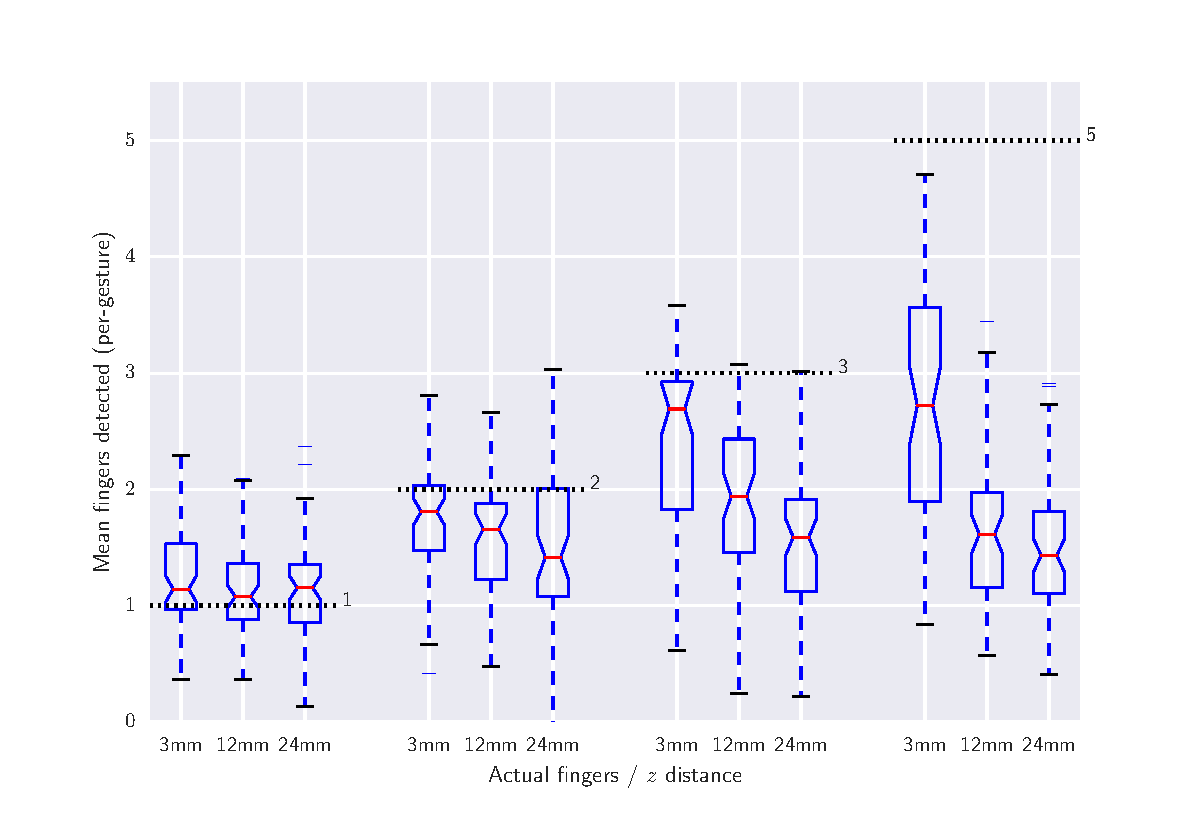
\includegraphics[width=1.0\linewidth]{images/boxplot_finger_distance.pdf}
    
    \caption{Average number of fingers detected by the touch sensor at different heights above the surface, averaged over all gestures. Dashed lines indicate
        the true number of fingers present. The Box plots include bootstrapped uncertainty notches for the median. It is clear that the device is biased toward
        undercounting fingers, particularly at higher $z$ distances.
    }
    
    % use the notation fig:name to cross reference a figure
    \label{fig:boxplot}
\end{figure}


%==================================================================================================================================
\chapter{Conclusion}
Summarise the whole project for a lazy reader who didn't read the rest (e.g. a prize-awarding committee).
\section{Guidance}
\begin{itemize}
    \item
          Summarise briefly and fairly.
    \item
          You should be addressing the general problem you introduced in the
          Introduction.
    \item
          Include summary of concrete results (``the new compiler ran 2x
          faster'')
    \item
          Indicate what future work could be done, but remember: \textbf{you
              won't get credit for things you haven't done}.
\end{itemize}

%==================================================================================================================================
%
%
%==================================================================================================================================
%  APPENDICES

\begin{appendices}


    \chapter{Appendices}
    
    
    Typical inclusions in the appendices are:
    
    \begin{itemize}
        \item
              Copies of ethics approvals (required if obtained)
        \item
              Copies of questionnaires etc. used to gather data from subjects.
        \item
              Extensive tables or figures that are too bulky to fit in the main body of
              the report, particularly ones that are repetitive and summarised in the body.
              
        \item Outline of the source code (e.g. directory structure), or other architecture documentation like class diagrams.
              
        \item User manuals, and any guides to starting/running the software.
              
    \end{itemize}
    
    \textbf{Don't include your source code in the appendices}. It will be
    submitted separately.
    
\end{appendices}

%==================================================================================================================================
%   BIBLIOGRAPHY

% The bibliography style is abbrvnat
% The bibliography always appears last, after the appendices.

\bibliographystyle{abbrvnat}

\bibliography{l4proj}

\end{document}
